\section*{ÔN TẬP KIỂM TRA CUỐI KÌ 2 - ĐỀ 02}
\setcounter{ex}{0}\setcounter{bt}{0}
\Opensolutionfile{ans}[ans/ansBTTeX1]

\noindent\textbf{I. PHẦN TRẮC NGHIỆM:}
%Câu 1
\begin{ex}
Các bạn học sinh lớp 11A1 trả lời $40$ câu hỏi trong một bải kiểm tra. Kết quả được thống kê ở bảng sau:
\begin{center}
\begin{tabular}{|c|c|c|c|c|c|}
\hline
Số câu đúng & $[16;21)$ & $[21;26)$ & $[26;31)$ & $[31;36)$& $[36;41)$ \\
\hline
Số học sinh & $4$ & $6$ & $8$ & $18$ & $4$\\
\hline
\end{tabular}
\end{center}
Giá trị đại diện của nhóm thứ $2$ là
\choice
{\True $23{,}5$}
{$21$}
{$33{,}5$}
{$26$}
\end{ex}
%Câu 2
\begin{ex}
Cho $A$, $B$ là hai biến cố xung khắc. Đẳng thức nào sau đây đúng?
\choice
{\True $P\left(A\cup B\right)=P(A)+P(B)$}
{$P\left(A\cup B\right)=P(A) \cdot P(B)$}
{$P\left(A\cup B\right)=P(A)-P(B)$}
{$P\left(A\cap B\right)=P(A)+P(B)$
}
\end{ex}
%Câu 3
\begin{ex}
Cho số thực $a$ dương thỏa mãn $\sqrt[3]{a^2}\colon \sqrt{a^3}=a^m$. Tìm giá trị của $m$.
\choice
{$1$}
{$\dfrac{13}{6}$}
{$\dfrac{5}{6}$}
{\True $-\dfrac{5}{6}$}
\end{ex}
%Câu 4
\begin{ex}
Với $a$ là số thực dương tùy ý, $\log_3(3a)$ bằng
\choice
{$1-\log_3a$}
{$3+\log_3a$}
{$3\log_3a$}
{\True $1+\log_3a$}
\end{ex}
%Câu 5
\begin{ex}
Tập xác định của hàm số $y=\log_3(x-4)$ là
\choice
{\True $\left(4;+\infty\right)$}
{$\left(-\infty ;4\right]$}
{$\left(-\infty ;4\right)$}
{$\left[4;+\infty\right)$}
\end{ex}
%Câu 6
\begin{ex}
Tập nghiệm $S$ của bất phương trình $\log_2(x-1)<3$ là
\choice
{$S=\left(-\infty ;9\right)$}
{$S=\left(-\infty ;10\right)$}
{$S=(1;10)$}
{\True $S=(1;9)$}
\end{ex}
%Câu 7
\begin{ex}
Cho hàm số $y=f(x)$ có đạo hàm tại $x_0$ là $f'\left(x_0\right)$. Mệnh đề nào sau đây sai?
\choice
{$f'\left(x_0\right)= \lim \limits_{x\to x_0} \,\dfrac{f(x)-f\left(x_0\right)}{x-x_0}$}
{$f'\left(x_0\right)= \lim \limits_{h \to 0} \,\dfrac{f\left(x_0-h\right)-f\left(x_0\right)}{h}$}
{$f'\left(x_0\right)= \lim \limits_{h\to 0} \,\dfrac{f\left(x_0+h\right)-f\left(x_0\right)}{h}$}
{\True $f'\left(x_0\right)= \lim \limits_{x\to x_0} \,\dfrac{f\left(x+x_0\right)-f\left(x_0\right)}{x-x_0}$}
\end{ex}
%Câu 8
\begin{ex}
Cho hàm số $y=\dfrac{1}{4}x^4-3x^2-2021x+2022$. Giá trị $y'=x^4-6x^2-2021$ bằng
\choice
{\True $6$}
{$3$}
{$-2$}
{$-6$}
\end{ex}
%Câu 9
\begin{ex}
Đạo hàm của hàm số $y=-2x^5+4\sqrt{x}$, $(x>0)$ bằng biểu thức nào dưới đây?
\choice
{$-10x^4+\dfrac{1}{\sqrt{x}}$}
{$-10x^4+\dfrac{4}{\sqrt{x}}$}
{\True $-10x^4+\dfrac{2}{\sqrt{x}}$}
{$-10x^4-\dfrac{1}{\sqrt{x}}$}
\end{ex}
%Câu 10
\begin{ex}
Đạo hàm cấp hai của hàm số $y=x^5$ là
\choice
{\True $20x^3$}
{$5x^4$}
{$5x^3$}
{$25x^3$}
\end{ex}
%Câu 11
\begin{ex}
Cho hàm số $y=2\sin x-3\cos x$ có đạo hàm cấp hai $y''=a\sin x+b\cos x$. Khi đó $S=2a+b$ có kết quả bằng
\choice
{$S=1$}
{$S=7$}
{\True $S=-1$}
{$S=-7$}
\end{ex}
%Câu 12
\begin{ex}
Cho hình hộp chữ nhật $ABCD \cdot MNPQ$, đường thẳng nào dưới đây vuông góc với đường thẳng$AD$?
\choice
{$BC$}
{\True $AB$}
{$NP$}
{$CM$}
\end{ex}
%Câu 13
\begin{ex}
Trong không gian, cho hai đường thẳng phân biệt $a,b$ và mặt phẳng $(P)$, với $a\perp (P)$. Mệnh đề nào SAI trong các mệnh đề sau?
\choice
{\True Nếu $b \parallel a$ thì $b \parallel (P)$}
{Nếu $b \parallel a$ thì $b\perp (P)$}
{Nếu $b\perp (P)$ thì $b \parallel a$}
{Nếu $b \parallel (P)$ thì $b \perp a$}
\end{ex}
%Câu 14
\begin{ex}
Cho hình chóp $S.ABCD$ có đáy $ABCD$ là tứ giác lồi và $SA\perp (ABCD)$. Góc giữa $SB$ và mặt phẳng $(ABCD)$ là:
\choice
{\True $\widehat{SBA}$}
{$\widehat{SCA}$}
{$\widehat{SAB}$}
{$\widehat{SDA}$}
\end{ex}
%Câu 15
\begin{ex}
Cho hình chóp $S.ABC$ có $SA\perp (ABC)$. Biết đáy$ABC$ là tam giác vuông tại $B$ và $M$ là trung điểm của $BC$. Mặt phẳng nào sau đây vuông góc với mặt phẳng $(SBC)$.
\choice
{$(ABC)$}
{\True $(SAB)$}
{$(SAC)$}
{$(SAM)$}
\end{ex}
%Câu 16
\begin{ex}
Cho hình chóp tứ giác $S.ABCD$ có đáy $ABCD$ là hình vuông cạnh $a$, $SB=a\sqrt{5}$ và $SA\perp (ABCD)$. Khoảng cách từ $S$ đến $(ABCD)$ bằng
\choice
{$a$}
{$a\sqrt{2}$}
{$4a$}
{\True $2a$}
\end{ex}
%Câu 17
\begin{ex}
Cho hình chóp tứ giác $S.ABCD$ có đáy $ABCD$ là hình chữ nhật và $SA\perp (ABCD)$. Khoảng cách giữa đường thẳng $BC$ và mặt phẳng $(SAD)$ là
\choice
{$BD$}
{\True $AB$}
{$SB$}
{$SC$}
\end{ex}
%Câu 18
\begin{ex}
Khối lăng trụ có diện tích đáy bằng $a^2$ và chiều cao bằng $3a$. Thể tích của khối lăng trụ đó bằng
\choice
{$\dfrac{a^3}{3}$}
{$a^3$}
{\True $3a^3$}
{$9a^3$}
\end{ex}
%Câu 19
\begin{ex}
Khối chóp cụt đều có chiều cao bằng $3a$, diện tích hai đáy lần lượt bằng $a^2$ và $4a^2$. Thể tích của khối chóp cụt đều đó bằng
\choice
{\True $7a^3$}
{$\dfrac{7a^3}{3}$}
{$\dfrac{a^3}{3}$}
{$21a^3$}
\end{ex}
%Câu 20
\begin{ex}
Cho khối chóp có diện tích đáy bằng $2a^2$ và chiều cao bằng $4a$. Thể tích của khối chóp đã cho bằng
\choice
{$8a^3$}
{\True $\dfrac{8a^3}{3}$}
{$\dfrac{2a^3}{3}$}
{$6a^3$}
\end{ex}
%Câu 21
\begin{ex}
Điều tra về mức lương của giáo viên tại một trường tư thục thu được kết quả như sau:
\begin{center}
\begin{tabular}{|c|c|c|c|c|c|}
\hline
Lương (triệu đồng) & $[10;12)$ & $[12;14)$ & $[14;16)$ & $[16;18)$& $[18;20)$ \\
\hline
Số giáo viên & $5$ & $13$ & $7$ & $3$ & $2$\\
\hline
\end{tabular}
\end{center}
Chọn khẳng định đúng trong các khẳng định sau:
\choice
{\True Mốt của mẫu số liệu trên thuộc nhóm thứ 2}
{Trung bình lương giáo viên trong trường là $16{,}5$ triệu đồng}
{Nhóm chứa trung vị là $[16;18)$}
{Tứ phân vị thứ ba là $15{,}56$}
\end{ex}
%Câu 22
\begin{ex}
Cho $A$, $B$ là hai biến cố xung khắc. Biết $P(A)=\dfrac{1}{5}$, $P\left(A\cup B\right)=\dfrac{1}{3}$. Tính $P(B)$.
\choice
{$\dfrac{3}{5}$}
{$\dfrac{8}{15}$}
{\True $\dfrac{2}{15}$}
{$\dfrac{1}{15}$}
\end{ex}
%Câu 23
\begin{ex}
Cho hai số thực dương $a,b$. Biết $\log_2\dfrac{\sqrt{4a^3b}}{ab}=1+x\log_2a+y\log_4b\quad (x,y\in \mathbb{Q})$.Tính $x+y$
\choice
{$1$}
{$-\dfrac{1}{4}$}
{$-1$}
{\True $0$}
\end{ex}
%Câu 24
\begin{ex}
\immini{Đồ thị hình bên là đồ thị của hàm số nào?
\choice
{$y=\left(\sqrt{3}\right)^x$}
{$y=3^x$}
{\True $y=\left(\dfrac{1}{3}\right)^x$}
{$y=\left(\dfrac{1}{4}\right)^x$}
}{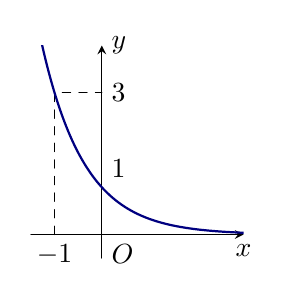
\begin{tikzpicture}[line join = round, line cap = round, >=stealth, scale = .6]
%Hệ trục Oxy và hàm số cần vẽ
\def\xmin{-1.5}     \def\xmax{3}
\def\ymin{-.5}       \def\ymax{4}
\def\f(#1){(1/3)^(#1)}
%Vẽ hệ trục
\draw[->] (\xmin,0)--(0,0) node[below right]{$O$}--(\xmax,0) node[below]{$x$};
\draw[->] (0,\ymin)--(0,\ymax) node[right]{$y$};
\draw[dashed] (-1,0)node[below]{$-1$}|-(0,3)node[right]{$3$} (0,1)node[above right]{$1$};
%Vẽ hàm số
\begin{scope}
\clip (\xmin,\ymin) rectangle (\xmax,\ymax);
\draw[smooth, thick, blue!50!black] plot[domain = \xmin:\xmax, samples = 200, variable=\x]({\x},{\f(\x)});
\end{scope}
\end{tikzpicture}}
\end{ex}
%Câu 25
\begin{ex}
Tìm số nghiệm nguyên của bất phương trình $\log_2^2x-8\log_2\sqrt{x}+3<0$.
\choice
{\True $5$}
{$1$}
{$7$}
{$4$}
\end{ex}
%Câu 26
\begin{ex}
Cho hàm số $f(x)=3x^3+4x^2-x-2$ có đồ thị $(C)$. Tìm hệ số góc của tiếp tuyến với đồ thị $(C)$ tại điểm có hoành độ $x_0=-2$.
\choice
{$-8$}
{$-53$}
{\True $19$}
{$17$}
\end{ex}
%Câu 27
\begin{ex}
Đạo hàm của hàm số $y=\sqrt{3x^2+4}$ là?
\choice
{$y'=\dfrac{1}{2\sqrt{3x^2+4}}$}
{$y'=\dfrac{x}{\sqrt{3x^2+4}}$}
{$y'=\dfrac{6x}{\sqrt{3x^2+4}}$}
{\True $y'=\dfrac{3x}{\sqrt{3x^2+4}}$}
\end{ex}
%Câu 28
\begin{ex}
Tính đạo hàm của hàm số $y=\left(x^2-2\right)(2x-1)$.
\choice
{$y'=4x$}
{$y'=3x^2-6x+2$}
{$y'=2x^2-2x+4$}
{\True $y'=6x^2-2x-4$}
\end{ex}
%Câu 29
\begin{ex}
Cho hàm số $y=\cos^2x$. Khi đó $y''\left(\dfrac{\pi }{3}\right)$ bằng:
\choice
{$2$}
{\True $1$}
{$-1$}
{$-2$}
\end{ex}
%Câu 30
\begin{ex}
Cho hình chóp $S.ABCD$ có $SA\perp (ABCD)$ và đáy là hình vuông. Khẳng định nào sau đây đúng?
\choice
{\True $BC\perp (SAB)$}
{$AC\perp (SAD)$}
{$AC\perp (SBD)$}
{$AC\perp (SAB)$}
\end{ex}
%Câu 31
\begin{ex}
Cho hình chóp $S.ABCD$ có $SA\perp (ABCD)$, $SA=a\sqrt{6}$. Biết đáy$ABCD$ là hình vuông tâm $O$ cạnh $2a$. Số đo góc phẳng nhị diện $\left[S, BD, A\right]$ là
\choice
{${{30}^\circ}$}
{${{45}^\circ}$}
{\True ${{60}^\circ}$}
{${{120}^\circ}$}
\end{ex}
%Câu 32
\begin{ex}
Cho hình lăng trụ tam giác đều $ABC.A'B'C'$ có độ dài cạnh đáy bằng $2a$ và cạnh bên bằng $3a$. Khoảng cách giữa hai đường thẳng $AB$ và $CC'$ bằng
\choice
{$2a$}
{\True $a\sqrt{3}$}
{$3a$}
{$a\sqrt{13}$}
\end{ex}
%Câu 33
\begin{ex}
Cho hình chóp $S.ABC$ có góc giữa các đường thẳng $SA, SB, SC$ và mặt phẳng $(ABC)$ cùng bằng $\alpha $. Tam giác $ABC$ nội tiếp đường tròn bán kính $R$. Khoảng cách từ điểm $S$ đến mặt phẳng $(ABC)$ bằng:
\choice
{$R\sin \alpha $}
{$R\cos \alpha $}
{\True $R\tan \alpha $}
{$R\cot \alpha $}
\end{ex}
%Câu 34
\begin{ex}
Cho hình chóp $S.ABC$, có $ABC$ là tam giác đều cạnh $a$, $SA$ vuông góc với đáy và $SA=a\sqrt{5}$. Tính thể tích $V$ của khối chóp $S.ABC$.
\choice
{$\dfrac{a^3\sqrt{3}}{12}$}
{$\dfrac{a^3\sqrt{15}}{4}$}
{\True $\dfrac{a^3\sqrt{15}}{12}$}
{$\dfrac{a^3\sqrt{5}}{4}$}
\end{ex}
%Câu 35
\begin{ex}
Cho hình lăng trụ đứng $ABC \cdot A'B'C'$, có đáy $ABC$ là tam giác vuông cân tại $C$ và $AB=2a$, góc giữa $A'C$ với mặt đáy bằng ${{45}^\circ}$. Tính thể tích khối lăng trụ đã cho.
\choice
{$4a^3$}
{$\dfrac{4a^3}{3}$}
{$\dfrac{a^3\sqrt{2}}{3}$}
{\True $a^3\sqrt{2}$}
\end{ex}

\noindent\textbf{II. PHẦN TỰ LUẬN}

%Câu 36
\begin{ex}
Tìm tập nghiệm của bất phương trình $3\log_{27} x <\log_{3}(x-2)+2.$
\end{ex}
%Câu 37
\begin{ex}
Cho hàm số $y=f(x)$ liên tục trên $\mathbb{R}$, có đồ thị $(C)$ và thỏa mãn $f\left(2x^3-1\right)+f(2-x)=x^6+5x^2-2x,\forall x\in \mathbb{R}$. Viết phương trình tiếp tuyến của đồ thị $(C)$ tại điểm $M$ có hoành độ $x_M=1$.
\end{ex}
%Câu 38
\begin{ex}
Cho khối chóp $S.ABC$ có đáy $ABC$ là tam giác vuông tại $C$, $BC=a;\widehat{BSC}=60^\circ $, cạnh $SA$ vuông góc với đáy, mặt phẳng $(SBC)$ tạo với $(SAB)$ góc $30^\circ $. Tính thể tích khối chóp $S.ABC$
\end{ex}
%Câu 39
\begin{ex}
Cho hình hộp $ABCD \cdot A'B'C'D'$ có $A'B$ vuông góc với mặt phẳng đáy $(ABCD)$, góc giữa $AA'$ và $(ABCD)$ bằng $45^\circ $. Khoảng cách từ $A$ đến các đường thẳng $BB'$ và $DD'$ bằng $1$. Góc giữa mặt $\left(BB'C'C\right)$ và mặt phẳng $\left(CC'D'D\right)$ bằng $60^\circ $. Tính thể tích khối hộp đã cho.
\end{ex}
\Closesolutionfile{ans}